\section{Testbed}

We analyze data from a large commercial building with 3 chillers, 4 air-handling units (AHU) and 179 thermal zones. A variable air volume (VAV) box modulates the airflow from the AHU to each zone. One AHU is associated to multiple VAVs. VAV modulation is achieved through a combination of two control actions: adjusting the air damper position (DMP) and regulating the local reheat valve (RVP) (Figure 1). The temperature in each zone ($T_{zone}$) is influenced also by the supply air temperature ($T_{sa}$) and flow ($FLW_{sa}$) coming from the AHU. All these points are monitored and recorded by the BAS, and represent the datasets used here. In addition, the room temperature is impacted by uncontrolled variables, such as weather (Toat is the outdoor air temperature), internal gains, and other thermal gains. This configuration is typical of a large number of buildings. The association between AHU and VAV is not stored in the BAS; however, for the purpose of the experiment, ground truth association was collected to verify the results of the proposed method. This paper explores different methods to discover the functional relationship (i.e the association) between the VAV box and the AHU that provides air to it.
 
 \begin{figure}[h!]

\centering
                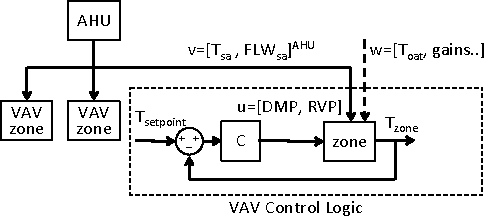
\includegraphics[width=0.45\textwidth]{./figs/ahudiagram.pdf}
                \caption{AHU and VAV configuration. On the right, the VAV control logic is represented. $T_{zone}$ is kept around the $T_{setpoint}$ by the control inputs $u=[DMP, RVP]$. $T_{zone}$ it is also influenced by parameters controlled by the AHU $(v=[T_{sa}, FLW_{sa}]^{AHU}$)  and external disturbances w=[$T_{oat}$, internal gains …].}
                \label{fig:ahudiagram}
\end{figure}
